\chapter{Introduction}

\section{Motivation}
May it be glorious space battles with lasers blasting around, or a mountain-high gorilla wrestling a even bigger lizard, modern rendering technologies present our craziest fantasies to our eyes as if they are happening right in front of us. The contemporary film and television industry is highly dependent on this ability of rendering photorealistic images, and alongside the pursuit of wilder stories and imaginations, the scenes to be rendered are becoming increasingly complex and arbitrary.

Despite its importance, the task of photorealistic rendering has a computational cost that is matched by few others. As an example, recent Disney title films could require hundreds of CPU hours just to synthesize a single frame \cite{hyperion}. This immense cost is explained by the fact that there are complex interactions between light rays and scene geometry, and the rendering algorithm must comprehensively and accurately simulate these interactions in order to obtain a realistic image. 

This project studies two orthogonal approaches that boost the efficiency of rendering. Firstly, this project utilizes GPUs (Graphics Processing Units), whose massively parallel architectures allow a large amount of pixels to be processed at the same time. Secondly, from an algorithmic perspective, the project explores how reinforcement learning can be used to guide the renderer to focus on the ``important'' parts of the scene. The project shows that both methods are indeed effective ways of improving rendering efficiency.

\section{Related Work}

The study of computer graphics began almost as soon as computers with screens were manufactured. In 1980, Whitted \cite{whitted} proposed the algorithm known as \textit{ray-tracing}, which is the algorithmic foundation of almost all photorealistic rendering algorithms used today. However, the version of ray-tracing described by Whitted was not based on a physically plausible model of light, and consequently the images generated were not yet photorealistic. 

The age of photorealism began in 1986 with the visionary work of Kaijiya \cite{rendering_equation}. This paper introduced an integral equation known as \textit{the rendering equation}, which models the energy carried by light rays in a physically correct manner. Programs that produce images by computing solutions to this equation are called physically based renderers, and this method have since become the focus of decades of rendering research. In addition, Kaijiya's paper also described a variant of the ray-tracing algorithm known as \textit{path-tracing}, which solves the rendering equation using the technique of Monte-Carlo integration. This algorithm is still the core of most of the photorealistic renderers developed and used today, including the renderer implemented in this project.

Path-tracing is a powerful algorithm, but it is too costly to be used for real-time rendering applications\footnote{until perhaps, very recently. See NVIDIA RTX.} such as video games. As a result, real-time applications take a fundamentally different approach to rendering known as rasterization. Modern rasterization-based rendering pipelines can be very-fast: they can render tens or even hundreds of frames per second. However, despite the fact that a range of algorithms \cite{fernando2005percentage,sloan2002precomputed,hanrahan1991rapid} exist that aims to make rasterization based algorithms as physically-correct as possible, the images produced by these renderers are still easily recognizable as computer generated. Thus, when the need for image quality dominates that for rendering speed, path-tracing is still the better choice. Notice that however, modern GPUs are designed to optimize for rasterization-based pipelines\footnote{Again, this is beginning to change with NVIDIA RTX.} and not for ray-tracing algorithms. 

In ray-tracing, one of the most costly operations is ray-scene intersection. Intuitively, this is the task of finding the first intersection point between a light ray and the geometries in the scene. A naive linear search across all geometries is of course unacceptably slow, and a range of accelerating data structures have been created. This project employs the data structure of Bounding Volume Hierarchies (BVH), which recursively divides the scene into a tree of axis-aligned bounding boxes. Due to their recursive nature, the construction and traversal of these structures are difficult tasks on GPUs. For this reason, this project studied and implemented a series of GPU BVH techniques published by NVIDIA \cite{bvh_build,bvh_optimize,bvh_traversal}.


Ever since the introduction of path-tracing, a variety of algorithms that builds on top of path-tracing have emerged. The most famous ones include bi-direction path-tracing \cite{veach1997robust}, Metropolis light transport \cite{veach1997robust,kelemen2002simple}, energy redistribution path-tracing \cite{cline2005energy}, and gradient-domain path-tracing \cite{kettunen2015gradient}. One particularly interesting variant, which uses reinforcement learning to guide the generation of light rays \cite{RLPT}, is studied and implemented in this project. 

One renderer of particular value to the graphics community is the \texttt{pbrt} renderer. Not only is this renderer open-source, it is also accompanied by an entire book \cite{pharr2016physically} which happens to be the most authoritative textbook of physically based rendering. Moreover, because of its popularity, there is a large collection of beautiful scenes defined using \texttt{pbrt}'s input file format. For these reasons, this project decided to support \texttt{pbrt}'s scene definition files, which allows this project to be benchmarked and compared against \texttt{pbrt}.

Most of the ray-tracing renderers used tody, including \texttt{pbrt}, runs on the CPU. However, there is a GPU ray-tracing system known as OptiX \cite{parker2010optix}, which is becoming increasingly popular. Developed by the GPU manufacturer NVIDIA, OptiX is heavily optimized, and provides a friendly ray-tracing library for developers. One famous renderer which uses OptiX as a backbone is the \texttt{Mitsuba} renderer\footnote{There is also an upcoming 4th version of \texttt{pbrt}, which also supports GPU via OptiX. However, the beta version is still unstable at the time this thesis is written.}. The GPU rendering routines of this project are implemented from scratch, and its performance will be compared against \texttt{Mitsuba} (and therefore OptiX).

\section{Project Outline}
This project focuses on the GPU parallelization of ray-tracing algorithms for the efficient rendering of photorealistic images. A fully-featured GPU renderer is created, which supports a wide range of geometries, materials, and light sources. At the heart of the renderer are efficient implementations of two algorithms: the original path-tracing algorithm, and a variant of path-tracing guided by reinforcement learning. 

To maximize the efficiency of path-tracing, this project implemented state-of-the-art methods of performing ray-scene intersection detection. These includes algorithms for constructing BVH trees in parallel, optimizing the structure of constructed BVHs, and recursion-free methods of tree traversal. The project also makes numerous optimizations that reduce control flow divergences and memory access latencies, so that the resulting implementation maximally utilizes the parallel architecture of GPUs.  

This project made the observation that in certain lighting scenarios, the original path-tracing algorithm struggles to converge to a noiseless solution. To alleviate this problem, the project implements a variant of path-tracing, where reinforcement learning is used to guide the selection of light rays. The project investigates how the architecture of the GPU interacts with various aspects of the reinforcement learning routine, and implements a version that allows tens of thousands of GPU threads to efficiently cooperate during learning. 


The renderer created by this project is named \texttt{Cavalry}\footnote{The name is inspired by a character in a video game called Overwatch. The character goes by the name ``Tracer'', and refers to herself as the ``Cavalry''. Figure \ref{figure tracer} is a rendered image of her.}. It is created mainly using the C++ programing language on the CPU side, and the CUDA language for GPU computing. With a total of over 7 thousand lines, the complete source code of the software can be found at \url{https://github.com/AmesingFlank/Cavalry}, along with some additional information and screenshots.

\begin{figure}[H]
    \centering
    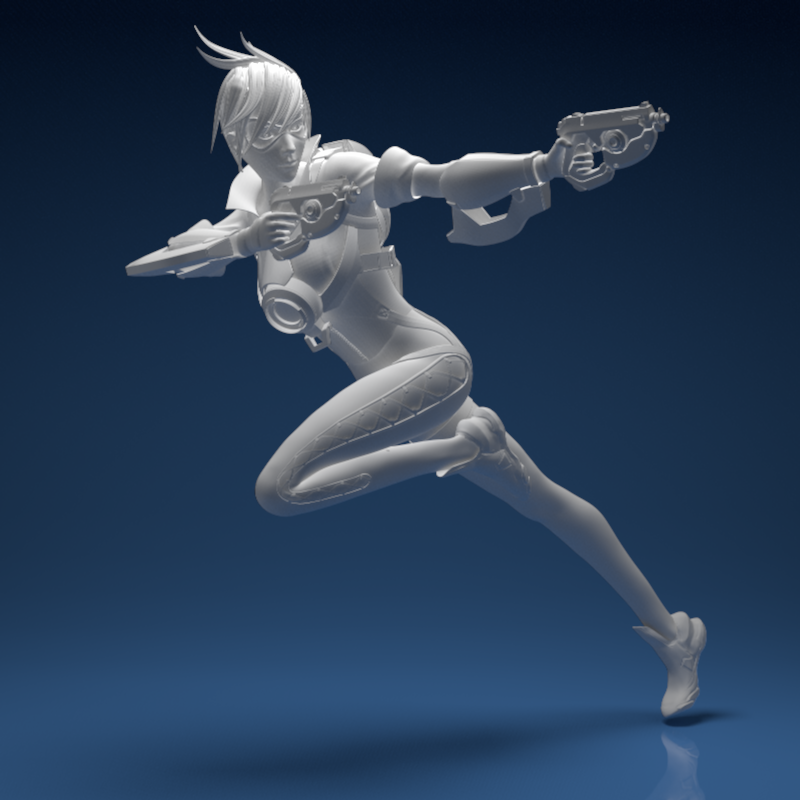
\includegraphics[height=14cm]{tracer copy.png}
    \caption{A video game character. Geometry created by \cite{tracer} and rendered using \texttt{Cavalry}.}
    \label{figure tracer}
\end{figure}